\subsection{DCGAN}
\label{sec:exp-dcgan}

We implement our baseline model in this section. The DCGAN is evaluated on cifar10. We present the evolution of the inception score in Figure \ref{fig:exp-dcgan-is} and both losses in Figure \ref{fig:exp-dcgan-losses}. These results serve as a reference for all our other experiments. The inception score seems to plateau around 5.8 with considerable deviations. Both the D and G losses are very unstable during training. \\
It is however important to note that losses can hardly be interpreted when treating with GANs, since the generator and discriminator are in a situation of competition where an improvement on the one leads to a deterioration on the other.
\begin{figure}[H]
    \centering
    \begin{subfigure}[t]{0.49\textwidth}
        \centering
		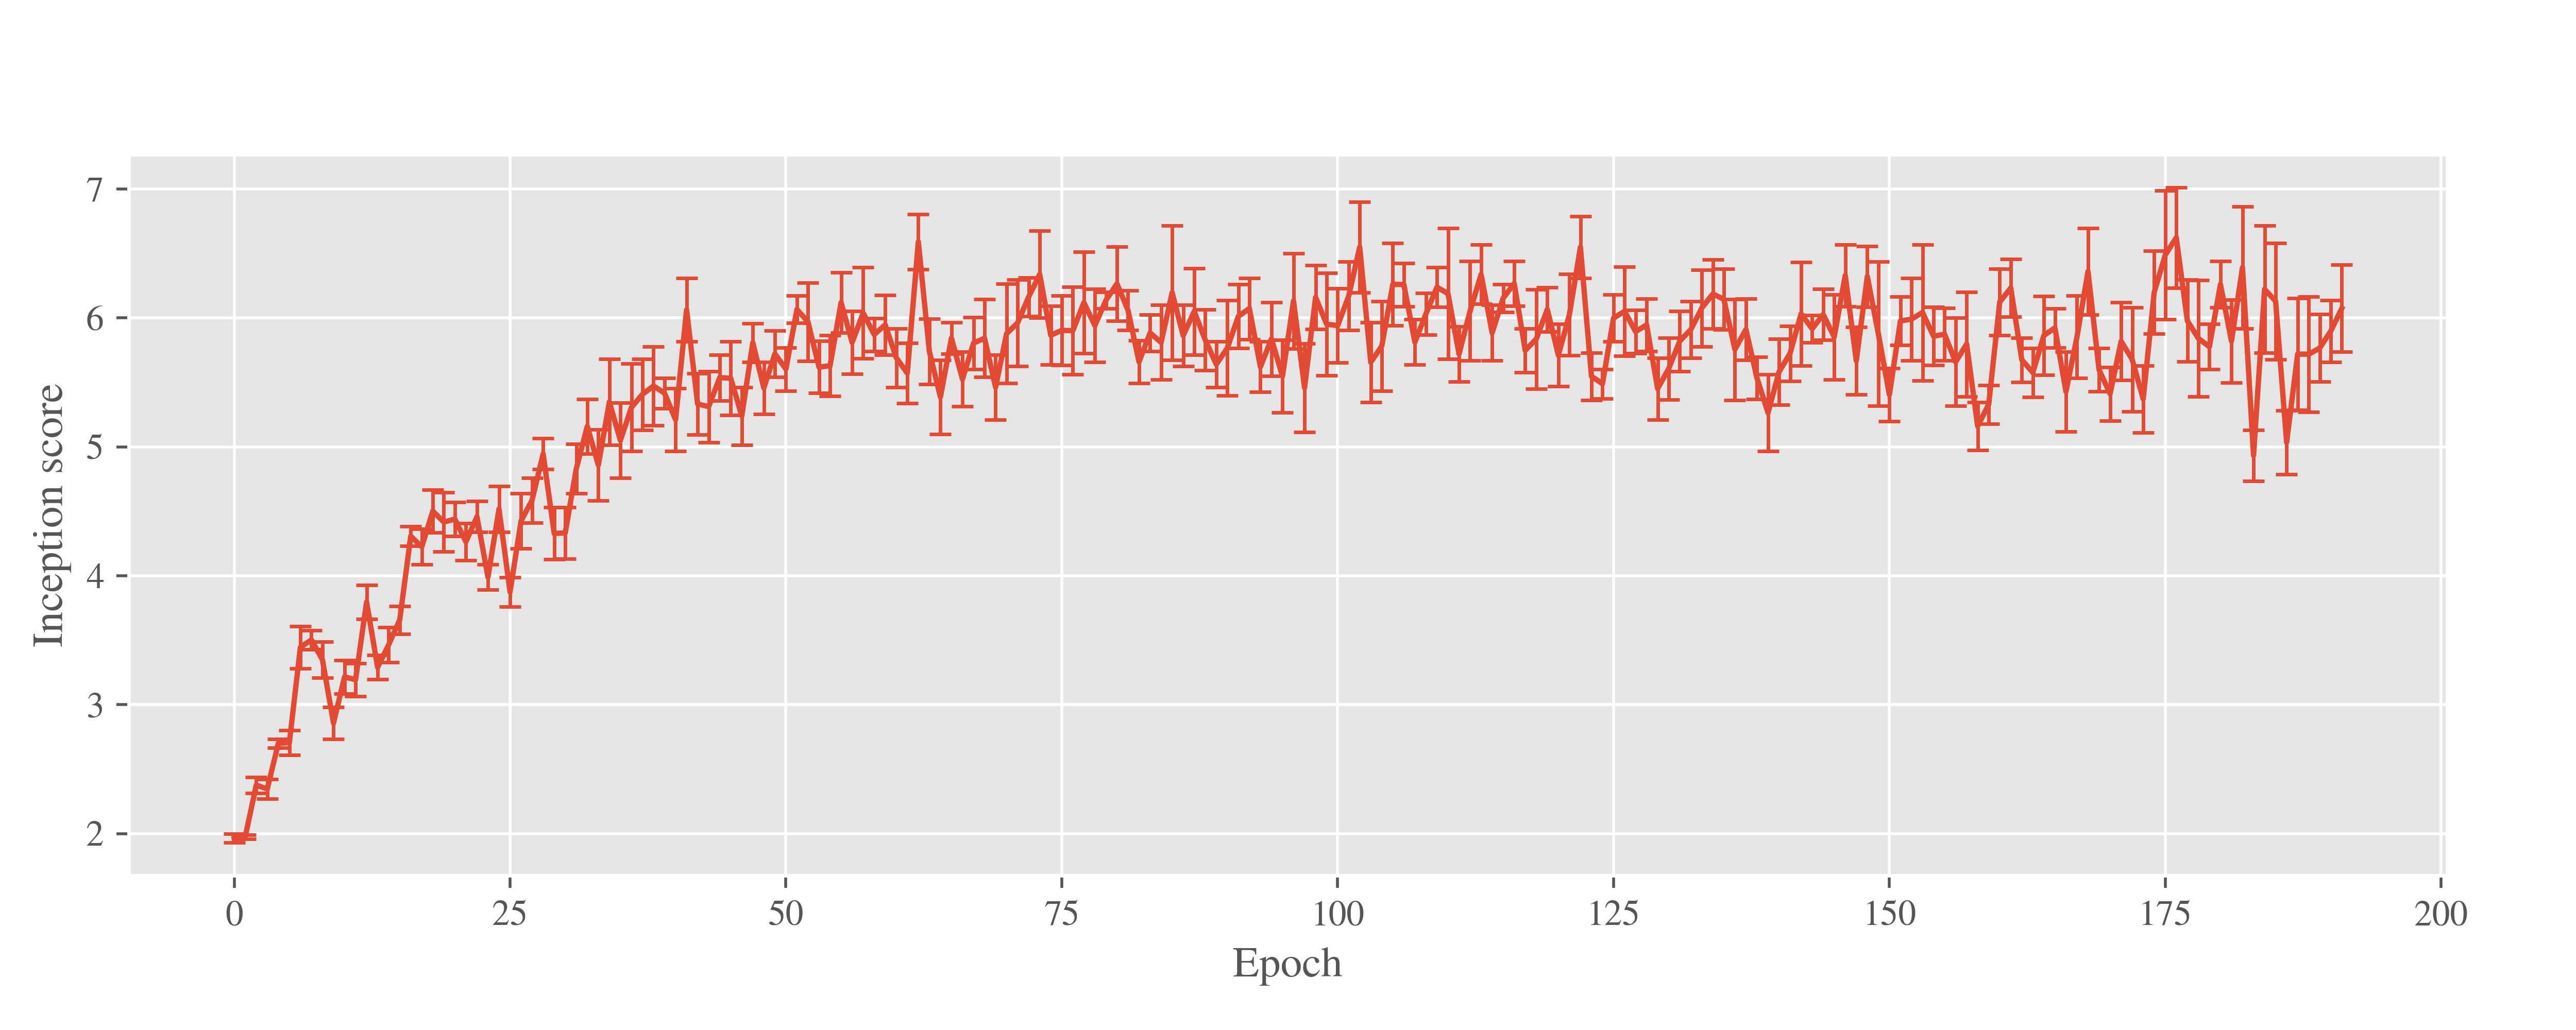
\includegraphics[width=\textwidth]{../code/results/figures/dcgan_cifar10_is.png}
		\caption{Inception score}
		\label{fig:exp-dcgan-is}
    \end{subfigure}
    \begin{subfigure}[t]{0.49\textwidth}
        \centering
        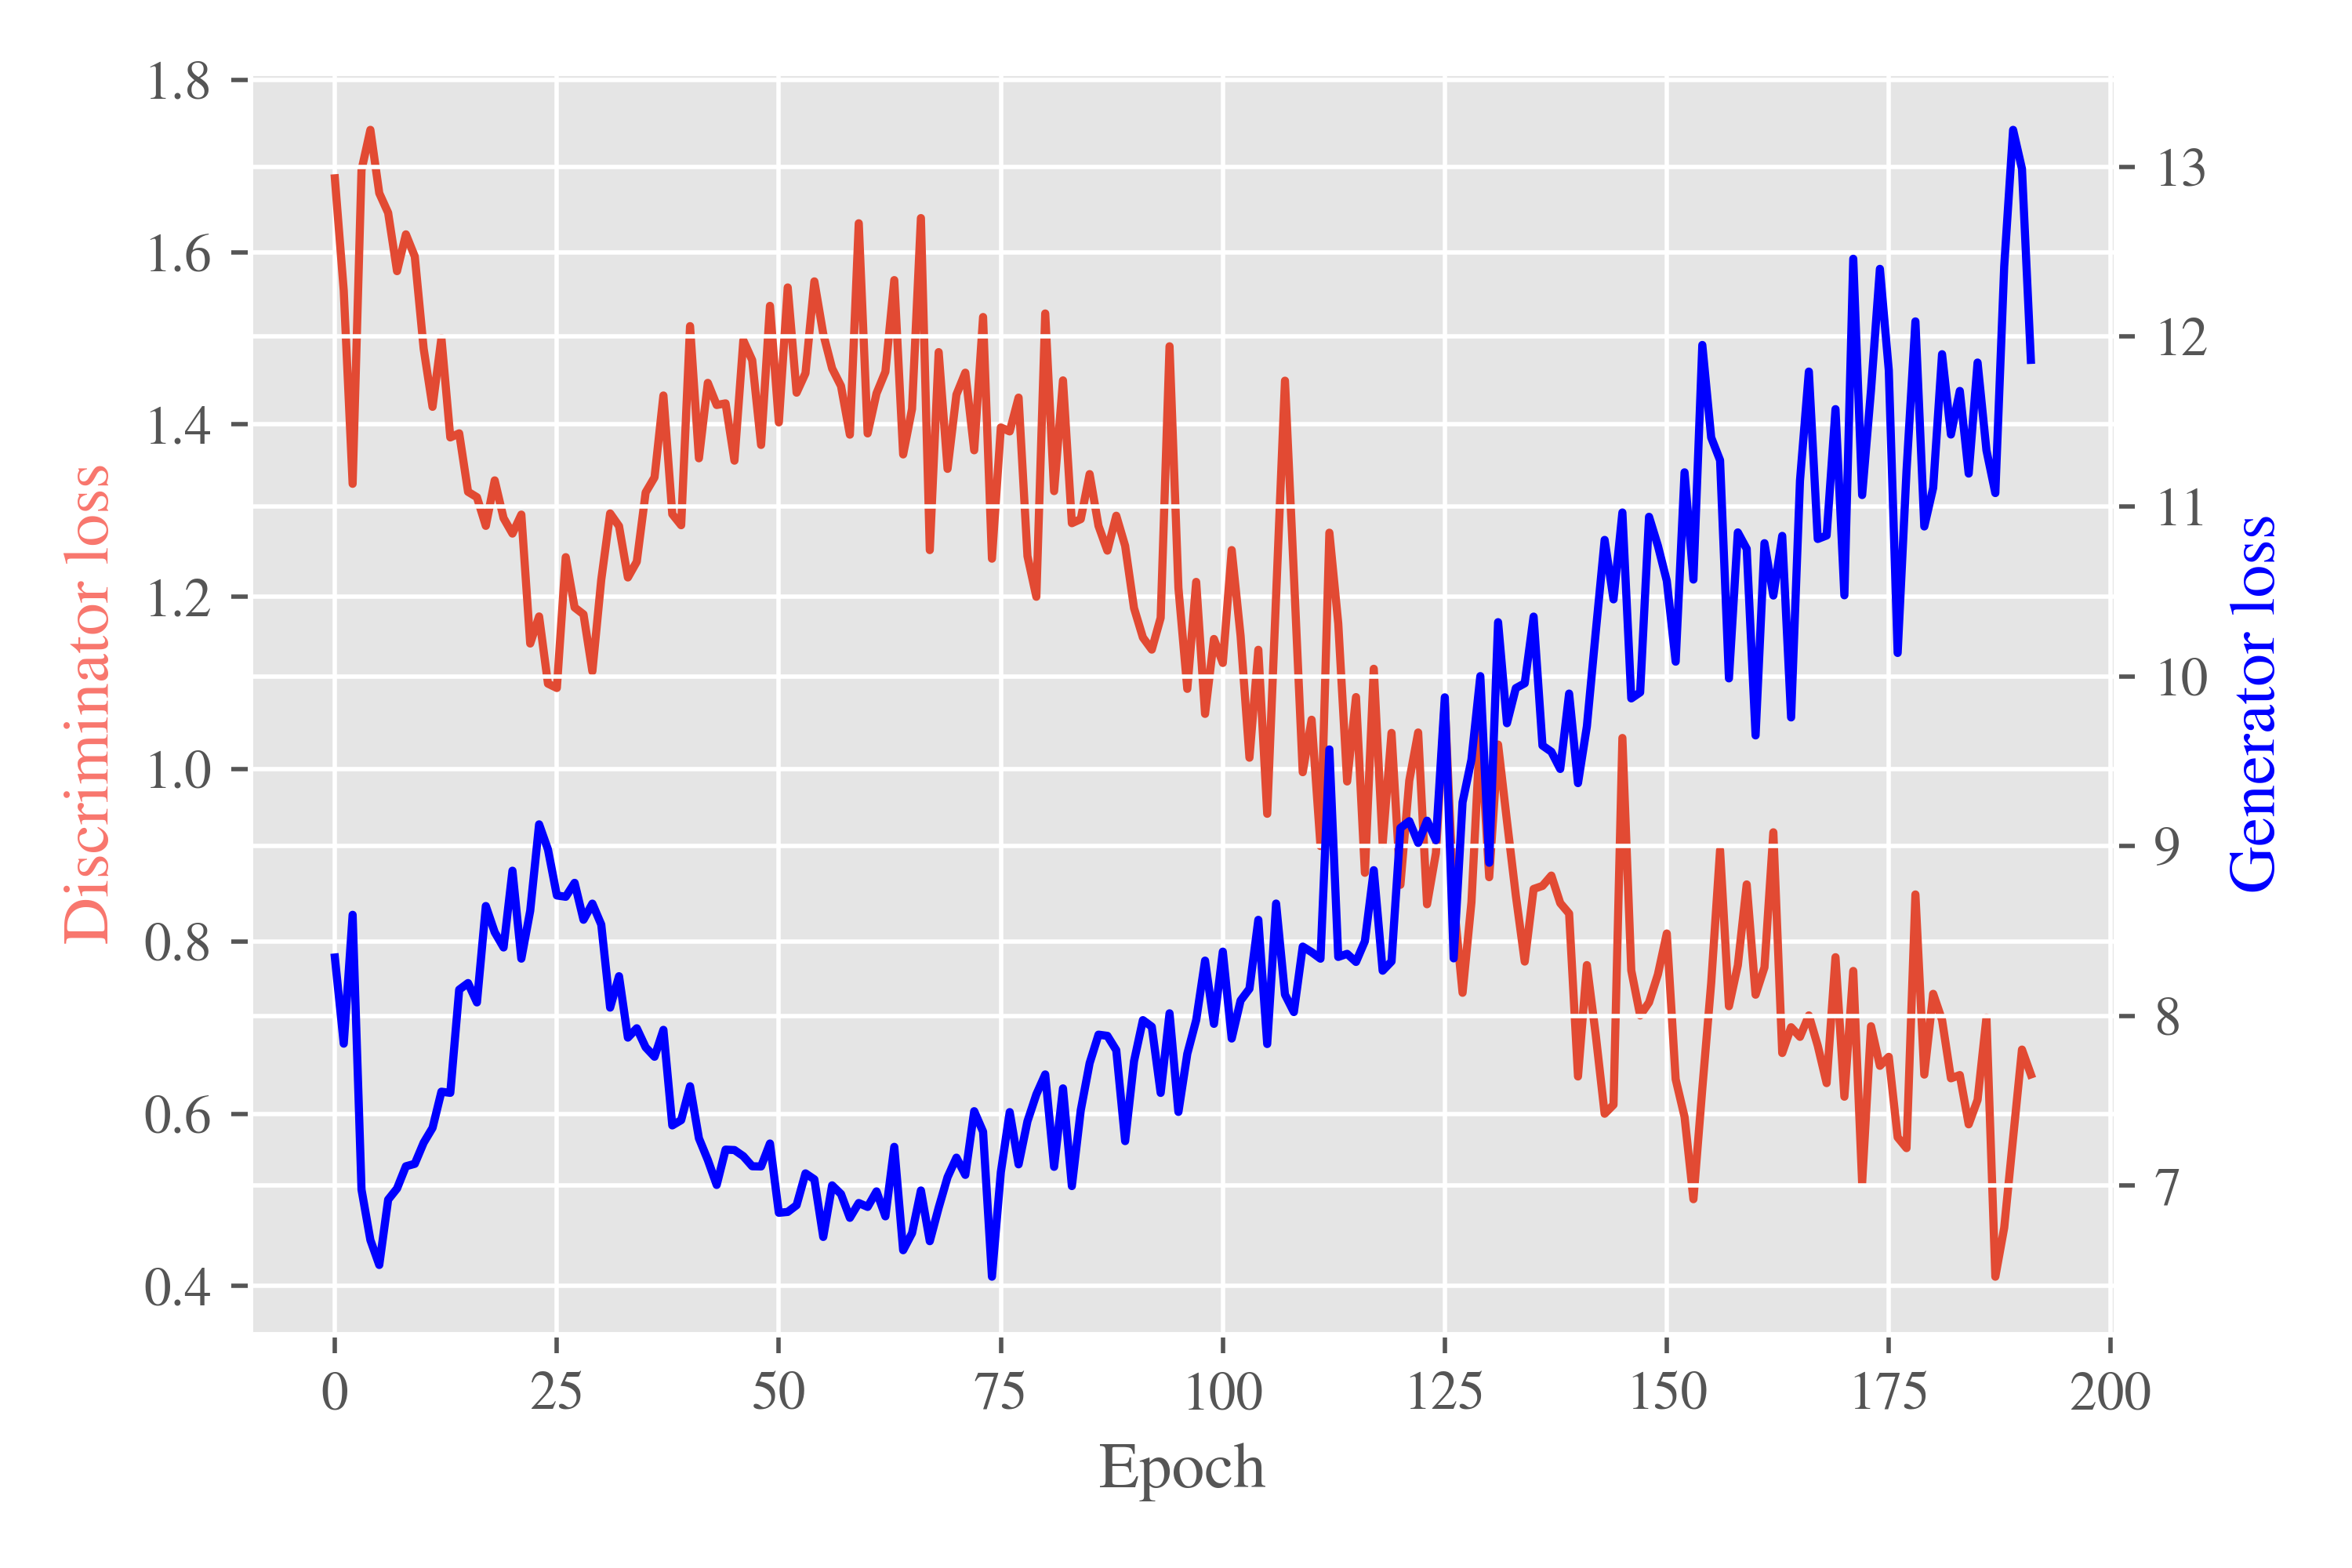
\includegraphics[width=\textwidth]{../code/results/figures/dcgan_cifar10_losses.png}
		\caption{Losses}
		\label{fig:exp-dcgan-losses}
    \end{subfigure}
    \caption{DCGAN - training on CIFAR10 over 190 epochs.}
\end{figure}
We conduct a visual inspection of the generated images and observe that many of them look alike, if not identical. This is a common phenomenon called mode collapse, in which the generator fails to learn the complete multimodal structure of the target data distribution and rather learns a subset of modes, allowing it to trick the discriminator but not to reproduce the target data distribution.